\section{Приложение Б}
Список смежности графа $G_1$:
\begin{verbatim}
2 2 5
4 1 3 4 5
2 2 7
1 2
2 1 2
2 7 8
2 3 6
1 6
\end{verbatim}

Список смежности графа $G_2$:
\begin{verbatim}
2 7 8
1 6
2 4 5
2 3 5
2 3 4
2 2 7
3 1 6 8
2 1 7
\end{verbatim}

Список смежности графа $G_3$:
\begin{verbatim}
5 2 4 10 11 12
2 1 4
4 6 7 9 11
3 1 2 5
4 4 6 7 9
4 3 5 7 8
3 3 4 8
1 6
3 3 5 10
3 1 9 11
3 1 3 10
1 1
\end{verbatim}

$G_4$ (\texttt{Examples/g4.txt}), изображённый на рис.~\ref{fig:g_5}:
\begin{verbatim}
6 2 5 6 16 17 20
6 1 3 6 7 17 18
6 2 4 7 8 18 19
6 3 5 8 9 19 20
6 1 4 6 9 10 20
6 1 2 5 7 10 11
6 2 3 6 8 11 12
6 3 4 7 9 12 13
6 4 5 8 10 13 14
6 5 6 9 11 14 15
6 6 7 10 12 15 16
6 7 8 11 13 16 17
6 8 9 12 14 17 18
6 9 10 13 15 18 19
6 10 11 14 16 19 20
6 1 11 12 15 17 20
6 1 2 12 13 16 18
6 2 3 13 14 17 19
6 3 4 14 15 18 20
6 1 4 5 15 16 20
\end{verbatim}
\begin{figure}[h!]
\begin{center}
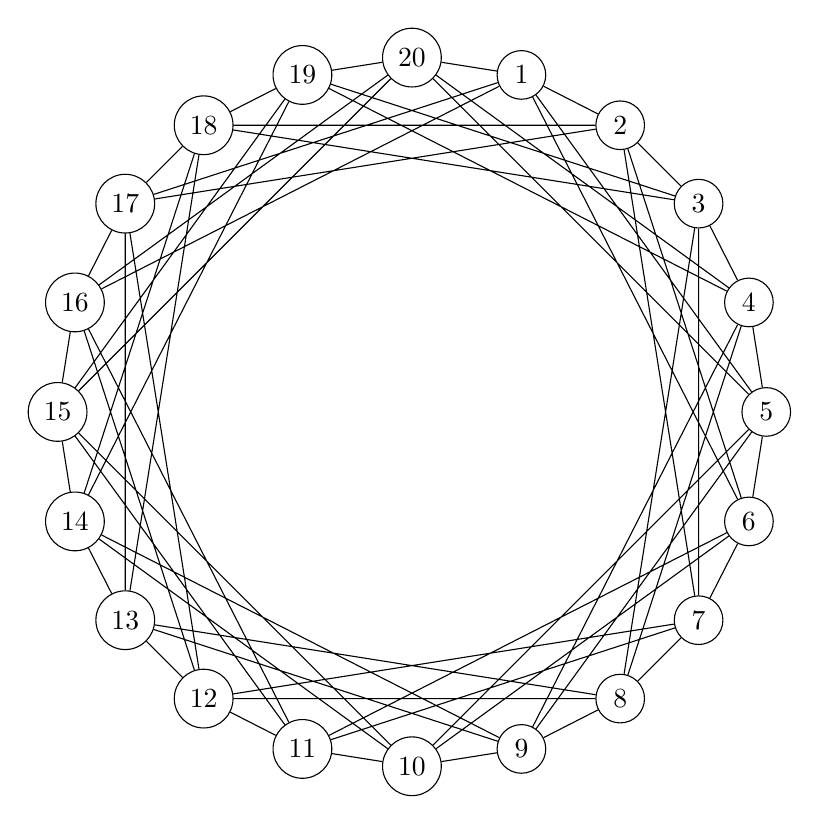
\begin{tikzpicture}
\tikzstyle{every node}=[draw,shape=circle];
\node (5) at ( 0:4.5) {$5$};
\node (4) at ( 18:4.5) {$4$};
\node (3) at (2*18:4.5) {$3$};
\node (2) at (3*18:4.5) {$2$};
\node (1) at (4*18:4.5) {$1$};
\node (20) at (5*18:4.5) {$20$};
\node (19) at (6*18:4.5) {$19$};
\node (18) at (7*18:4.5) {$18$};
\node (17) at (8*18:4.5) {$17$};
\node (16) at (9*18:4.5) {$16$};
\node (15) at (10*18:4.5) {$15$};
\node (14) at (11*18:4.5) {$14$};
\node (13) at (12*18:4.5) {$13$};
\node (12) at (13*18:4.5) {$12$};
\node (11) at (14*18:4.5) {$11$};
\node (10) at (15*18:4.5) {$10$};
\node (9) at (16*18:4.5) {$9$};
\node (8) at (17*18:4.5) {$8$};
\node (7) at (18*18:4.5) {$7$};
\node (6) at (19*18:4.5) {$6$};
\draw
(1) -- (2) (1) -- (5) (1) -- (6)
(2) -- (3) (2) -- (6) (2) -- (7)
(3) -- (4) (3) -- (7) (3) -- (8)
(4) -- (5) (4) -- (8) (4) -- (9)
(5) -- (6) (5) -- (9) (5) -- (10)
(6) -- (7) (6) -- (10) (6) -- (11)
(7) -- (8) (7) -- (11) (7) -- (12)
(8) -- (9) (8) -- (12) (8) -- (13)
(9) -- (10) (9) -- (13) (9) -- (14)
(10) -- (11) (10) -- (14) (10) -- (15)
(11) -- (12) (11) -- (15) (11) -- (16)
(12) -- (13) (12) -- (16) (12) -- (17)
(13) -- (14) (13) -- (17) (13) -- (18)
(14) -- (15) (14) -- (18) (14) -- (19)
(15) -- (16) (15) -- (19) (15) -- (20)
(16) -- (17) (16) -- (20) (16) -- (1)
(17) -- (18) (17) -- (1) (17) -- (2)
(18) -- (19) (18) -- (2) (18) -- (3)
(19) -- (20) (19) -- (3) (19) -- (4)
(20) -- (1) (20) -- (4) (20) -- (5)
;
\end{tikzpicture}
\caption{}\label{fig:g_5}
\end{center}
\end{figure}

$G_5$ (\texttt{Examples/g5.txt}), изображённый на рис.~\ref{fig:g_6}:
\begin{verbatim}
4 2 3 4 5
1 1
1 1
1 1
1 1
4 7 8 9 10
1 6
1 6
1 6
1 6
\end{verbatim}

\begin{figure}[h!]
\begin{center}
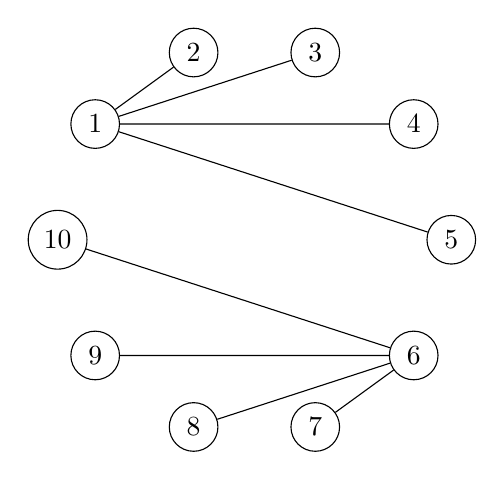
\begin{tikzpicture}
\tikzstyle{every node}=[draw,shape=circle];
\node (5) at ( 0:2.5) {$5$};
\node (4) at ( 36:2.5) {$4$};
\node (3) at (2*36:2.5) {$3$};
\node (2) at (3*36:2.5) {$2$};
\node (1) at (4*36:2.5) {$1$};
\node (10) at (15*36:2.5) {$10$};
\node (9) at (16*36:2.5) {$9$};
\node (8) at (17*36:2.5) {$8$};
\node (7) at (18*36:2.5) {$7$};
\node (6) at (19*36:2.5) {$6$};
\draw
(1) -- (2) (1) -- (3) (1) -- (4) (1) -- (5)
(6) -- (10) (6) -- (9) (6) -- (8) (6) -- (7)
;
\end{tikzpicture}
\caption{}\label{fig:g_6}
\end{center}
\end{figure}

